
%%%%%%%%%%%%%% 特徴量工学の説明 %%%%%%%%%%%%
\section{特徴量工学}
図\ref{fig:EEGfootmove}と図\ref{fig:EEGhandmove}はそれぞれ足の運動想起と手の運動想起を行った際の脳波である。
いずれも0秒以前は以前はディスプレイを注視した状態であり、0秒以降に運動想起を4秒間行っている。
電極の個数は64個用いられており、全ての電極の波形が表示されている。
足の運動想起が行われているのか手の運動想起が行われているのかを脳波の生データから識別するのは困難であることが分かる。
運動想起BCIの標準的な役割は、脳波信号から運動想起部位を識別することであるが、
そのためには脳波の生データに対して何らかの処理を施し、識別に有用な特徴を見出さねばならない。

\begin{figure}[t]
    \centering
    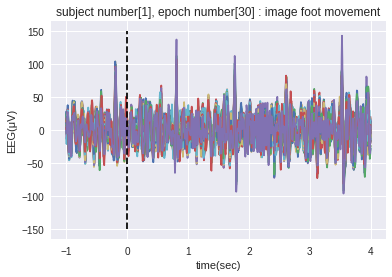
\includegraphics[width=9cm]{images/EEGfootmove.png}
    \caption{0秒〜4秒間に足の運動想起を行った際の脳波(EEG)}
    \label{fig:EEGfootmove}
\end{figure}
\begin{figure}[t]
    \centering
    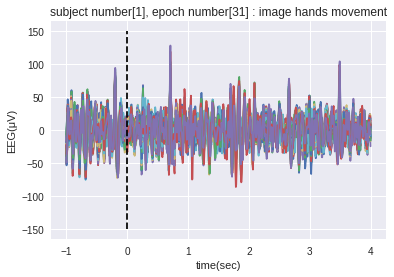
\includegraphics[width=9cm]{images/EEGhandmove.png}
    \caption{0秒〜4秒間に手の運動想起を行った際の脳波(EEG)}
    \label{fig:EEGhandmove}
\end{figure}
そこで、何らかの変換\(f(\cdot)\)を脳波信号\(x(t)\)に対して施すことで、
特徴量\(z=f(x(t))\)の獲得を目指すのが特徴量工学である。

\subsection{空間フィルタ}
脳波信号\(x(t)\in \mathbb R^D\)をとする。ここに\(D\)を電極の個数である。
まず初めに運動想起BCIに必要な電極について考慮する必要がある。
例えば足の動作に関する脳活動が脳波として観測される場合、頭皮上の全ての領域が対等に重要であるとは考えにくい。
従って、通常はBCIに必要となる電極の選定を行う。
足の動作に関する脳の領域は頭頂部に存在するため、脳波として観測される場合、
頭頂部に位置するCz電極が最も関係していると考えられる。
図\ref{fig:Cz}は足の運動想起を行った際のCz電極によって記録された脳波である。
しかし波形から足の運動想起を行っていることを判別する決定的な差異を見出すことは困難である。
\begin{figure}[t]
    \centering
    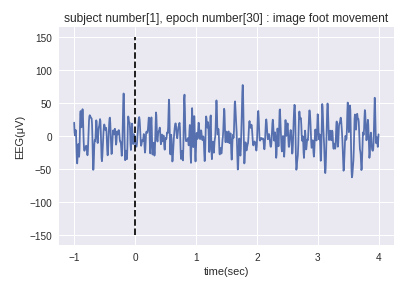
\includegraphics[width=9cm]{images/CzEEG.png}
    \caption{0秒〜4秒間に足の運動想起を行った際のCz電極の波形}
    \label{fig:Cz}
\end{figure}
理由としては、脳の頭頂部での神経活動によって生じている電位が、
必ずしも頭皮上の頭頂部にのみ伝搬するとは限らないからである。
電位を発生させている神経活動と電位を計測している電極との間には、頭蓋骨と皮膚があり、
電位の伝搬がどのように行われているかを完全に把握することは難しい。
ある程度空間的に広がりを持って電位が伝搬していると考えるのが自然である。
そこで計測された脳波に対して、スモールラプラシアンフィルタと呼ばれる空間フィルタが用いられることがある。
A電極によって計測された脳波を\(x_A(t)\)と表記すると、Cz電極に対するスモールラプラシアンフィルタが適用された脳波\(x_{smallCz}(t)\)は以下で表される。
\begin{equation}
    x_{smallCz}(t) = x_{Cz}(t) - \frac{1}{4}(x_{C1}(t) + x_{C2}(t) + x_{FCz}(t) + x_{CPz}(t))
\end{equation}
ラプラシアンフィルタは一般的に2次元配列\(X(i,j)\)に対して以下の計算によって二次差分を計算したものである。
\begin{equation}
    X(i,j) = -4X(i,j) + X(i-1,j) + X(i+1,j) + X(i,j-1) + X(i,j+1)
\end{equation}
二次差分フィルタは画像処理では輪郭検出のために用いられる処理であり、
空間的に配置された値が際立って変化する位置で大きな値を持つ配列を返す。
脳波に対してラプラシアンフィルタを適用する場合は、頭皮上の電極が2次元に配置されていると考え計算を行う。
信号に対する符号や絶対値はあまり重要視されていないためか、多くの場合は着目した電極の係数の符号を正とした計算が行われる。
図\ref{fig:Cz}はCz電極に対してスモールラプラシアンフィルタを用いた際の脳波である。
\begin{figure}[t]
    \centering
    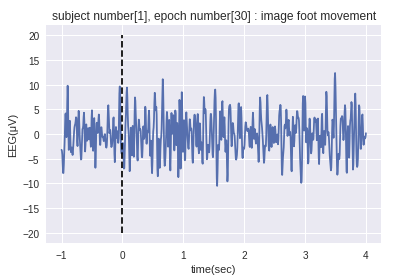
\includegraphics[width=9cm]{images/rapCzEEG.png}
    \caption{スモールラプラシアンフィルタを適用した際のCz電極の波形}
    \label{fig:Cz}
\end{figure}
スモールラプラシアンフィルタの処理によって必ずしも有効な特徴量が得られるとは限らないため、
適切な空間フィルタを獲得するために統計的なフィルタ設計方法が取られることもある。
特にIndependet Componet AnalysisとCommon Spatial Patternは、既に脳波解析に置いて確固たる地位を築いていると言える。
これらの手法に関しては後述する。




% \section{その他の手法}
% \subsection{スペクトログラムを特徴量とする手法}
% 運動想起型BCIでは、上記までに述べてきたCSPによる手法が非常に活発に議論されている。
% しかし、CSPによる手法は計測の際に多数の電極を用いる必要がある。
% 一方で実用上は電極が少なければ少ない程計測における負担は少なくなるため、
% 少数の電極のみを用いてBCIを構築する方法も研究がされている。
% 例として運動時、あるいは運動想起時には特定の頭皮領域に配置された電極において、
% 特定の周波数帯域にパワーの減少が生じること(事象関連脱同期)が知られているため、
% この現象に狙いを定めてBCIを構築する研究も盛んである。

% この手の手法の主な流れを示す。まず脳波信号を\(X \in \mathbb{R}^{M \times N}\)と表記する。ここに、\(M\)は電極の個数、\(N\)は計測時間点数である。
% 電極に対しての重み付け係数(空間フィルタ)$w \in \mathbb{R}^M$を何らかの方法で決定することで、
% \begin{equation*}
%     z = w^T X \in \mathbb{R}^N    
% \end{equation*}
% と変換する。次に$z$に対して短時間フーリエ変換${\cal F}(\cdot)$を行い、
% \begin{equation*}
%     A = {\cal F}(z) \in \mathbb{R}^{F\times N}
% \end{equation*}
% を獲得する。短時間フーリエ変換の代わりにウェーブレット変換などの時間周波数解析を用いる場合もある。
% スペクトログラム$A$から事象関連脱同期を見出すことができれば、ある特定の周波数帯域でのパワーを見張ることで運動の意図推定が可能となる。
% 実際、特定の周波数帯域のパワーに対して閾値を設けることで、運動意図推定を行う手法も提案されている。
% ただし、事象関連脱同期が生じる周波数帯域には個人差があることが想定されるため、スペクトログラム$A$に対して何らかの行列分解を用いて特徴量を取り出すことも提案されている。



% \subsection{Convolutional Neural Networks(ConvNets)}
% この手法に関しては\cite{deepconv}を参照されたい。